\documentclass[envcountsect,envcountsame,orivec,oribibl]{llncs}
% \documentclass[a4paper,UKenglish]{lipics}
% \documentclass[conference]{IEEEtran}
% \usepackage{mathtools}
\usepackage{amsmath,amssymb}
\usepackage[dvipdfm]{graphicx}
% \usepackage{xspace}
% \usepackage{hyperref}
\let\proof\relax
\let\endproof\relax
\usepackage{amsthm}
\usepackage{microtype}
\usepackage[all]{xy}

% \usepackage{mtpro}

\newcommand{\R}{\mathbb R}
\newcommand{\N}{\mathbb N}
\newcommand{\Z}{\mathbb Z}
\newcommand{\I}{\mathbb I}
\newcommand{\C}{\mathbb C}
\newcommand{\D}{\mathbb D}


\newcommand{\classonefont}[1]{\mathsf{#1}}
\newcommand{\classL}{\classonefont{L}}
\newcommand{\classFL}{\classonefont{FL}}
\newcommand{\classP}{\classonefont{P}}
\newcommand{\classFP}{\classonefont{FP}}
\newcommand{\classPP}{\classonefont{PP}}
\newcommand{\classSharpP}{\classonefont{\#P}}
\newcommand{\classPSPACE}{\classonefont{PSPACE}}
\newcommand{\classFPSPACE}{\classonefont{FPSPACE}}
\newcommand{\classNP}{\classonefont{NP}}
\newcommand{\classNC}{\classonefont{NC}}
\newcommand{\classFNC}{\classonefont{FNC}}
\newcommand{\classAC}{\classonefont{AC}}
\newcommand{\classFAC}{\classonefont{FAC}}
\newcommand{\classNumberP}{\classonefont{\#P}}
\newcommand{\classPH}{\classonefont{PH}}
\newcommand{\classCH}{\classonefont{CH}}
\newcommand{\classSigma}{\classonefont{\Sigma}}


\newcommand{\classtwofont}[1]{\text{\bfseries \sffamily \upshape #1}}
\newcommand{\classLtwo}{\classtwofont{L}}
\newcommand{\classFLtwo}{\classtwofont{FL}}
\newcommand{\classFNCtwo}{\classtwofont{FNC}}
\newcommand{\classFACtwo}{\classtwofont{FAC}}
\newcommand{\classPtwo}{\classtwofont{P}}
\newcommand{\classFPtwo}{\classtwofont{FP}}
\newcommand{\classPPtwo}{\classtwofont{PP}}
\newcommand{\classSharpPtwo}{\#\classtwofont{P}}
\newcommand{\classPSPACEtwo}{\classtwofont{PSPACE}}
\newcommand{\classFPSPACEtwo}{\classtwofont{FPSPACE}}
\newcommand{\classCHtwo}{\classtwofont{CH}}
\newcommand{\classFCHtwo}{\classtwofont{FCH}}


\newcommand{\deltabox}{\delta _\square}
\newcommand{\deltaboxLip}{\delta _{\square \mathrm L}}
\newcommand{\deltaboxCM}{\delta _{\square \mathrm{CM}}}
\newcommand{\deltaboxINV}{\delta _{\square \mathrm{INV}}}
\newcommand{\deltaTaylor}{\delta _{\mathrm{Taylor}}}
\newcommand{\id}{\mathrm{id}}
\newcommand{\rhoSigmastar}{\rho _{\Sigma ^*}}
\newcommand{\rhoD}{\rho _\D}
\newcommand{\rhoR}{\rho _\R}
\newcommand{\rhoI}{\rho _\I}
\newcommand{\rhoRunit}{\rho _\R|^{[0,1]}}
\newcommand{\rhoCSet}{\rho_{\C\mathrm{Set}}}


\newcommand{\redW}{\leq _{\mathrm W}}
\newcommand{\redm}{\leq _{\mathrm{m}}}
\newcommand{\redmF}{\leq _{\mathrm{mF}}}
\newcommand{\redB}{\leq _{\mathrm B}}
\newcommand{\redLW}{\redW ^{\classLtwo}}
\newcommand{\redLmF}{\redmF ^{\classLtwo}}
\newcommand{\redLB}{\redB ^{\classLtwo}}


\newcommand{\classLip}{\mathrm{CL}}
\newcommand{\classC}{\mathrm C}


\newcommand{\LM}{\varSigma ^{**}}

\newcommand{\probCVP}{\mathrm{CVP}}


\newcommand{\OpApply}{\mathit{Apply}}
\newcommand{\OpIVP}{\mathit{ODE}}
\newcommand{\OpCMFix}{\mathit{Fix}}
\newcommand{\OpINV}{\mathit{Inv}}
\newcommand{\OpCVP}{\mathrm{CVP}^2}
\newcommand{\OpPolyRoot}{\mathit{PolyRoot}}
\newcommand{\OpF}{\mathcal{F}}
\newcommand{\probDTIMEtwo}{\mathrm{DTIME}^2}
\newcommand{\probCVPtwo}{\mathrm{CVP}^2}


\newcommand{\dom}{\mathop{\rm dom}}
\newcommand{\depth}{\mathop{\rm depth}}


\newcommand{\OR}{\mathrm{OR}}
\newcommand{\NOT}{\mathrm{NOT}}
\newcommand{\AND}{\mathrm{AND}}
\newcommand{\FANOUT}{\mathrm{FAN-OUT}}

%% \newtheorem{theorem}{Theorem}[section]
%% \newtheorem{lemma}[theorem]{Lemma}
%% \newtheorem{corollary}[theorem]{Corollary}
%% \theoremstyle{definition}
%% \newtheorem{definition}[theorem]{Definition}
%% \newtheorem{example}[theorem]{Example}
%% \theoremstyle{remark}

\newcommand{\pcolon}{\mathpunct{\,:\subseteq}}

\title{Small complexity classes for computable analysis}
%% \author{\IEEEauthorblockN{Akitoshi Kawamura}
%% \IEEEauthorblockA{Department of Computer Science\\
%% University of Tokyo}
%% \and
%% \IEEEauthorblockN{Hiroyuki Ota}
%% \IEEEauthorblockA{Department of Computer Science\\
%% University of Tokyo}
%% }
\author{Akitoshi Kawamura\and Hiroyuki Ota}

\begin{document}

\maketitle

\begin{abstract}
Type-two Theory of Effectivity (TTE) provides a concrete and general framework for 
Computable Analysis. 
To refine it to polynomial-time computability 
while keeping as much generality as possible, 
Kawamura and Cook recently proposed a modification to TTE using 
machines that have random access to an oracle and 
run in time depending on the ``size'' of the oracle. 
They defined type-two analogues of 
$\classP$, $\classNP$, $\classPSPACE$ 
and applied them to real functions and operators. 
We further refine their model and study computation below $\classP$: 
type-two analogues of 
the classes $\classL$, 
$\classNC$, 
and $\classP$-completeness under log-space reductions.
The basic idea is 
to use second-order polynomials as resource bounds, 
as Kawamura and Cook did, 
but we need to make some nontrivial (yet natural, as we will argue) choices
when formulating small classes
in order to make them well-behaved. 
Most notably: 
we use a modification of the constant stack model 
of Aehlig, Cook and Nguyen for query tapes 
in order to allow sufficient oracle accesses without interfering with space bounds; 
representations need to be chosen carefully, as 
computational equivalence between them is now finer; 
uniformity of circuits must be defined 
with varying sizes of oracles taken into account. 
As prototypical applications, 
we recast several facts (some in a stronger form than was known) 
about the complexity of numerical problems 
into our framework. 
\end{abstract}

\section{Introduction}
\label{section: introduction}

Computable Analysis 
\cite{bhw,ko1991complexity,weihrauch00:_comput_analy}
studies problems 
involving real numbers, real functions and other objects in analysis
from the viewpoint of computability on digital machines. 
Elements of uncountable sets (such as real numbers) are
represented through approximations (such as sequences of rational numbers)
and processed by Turing machines. 
Such approximation can be 
presented to the machine 
as infinite strings on the tape 
or as oracles (i.e., functions taking strings to strings), 
and this choice does not make much difference 
as long as we only discuss computability. 
But when we want to pay attention to bounds on time and space, 
Kawamura and Cook \cite{kawamura2012complexity} recently pointed out that 
it is more convenient to use oracles with random access, 
and moreover, to allow the running time 
to depend on the ``size'' of the oracle. 
Employing \emph{type-two complexity theory} and 
using \emph{second-order polynomials} to bound time and space, 
they formulated analogues of complexity classes 
$\classP$, $\classNP$, $\classPSPACE$ and 
applied them to some typical operators in analysis. 
The basic definitions will be reviewed in Section~\ref{section: computable analysis}. 

One benefit of this was
a greater variety of objects for which we can define complexity. 
For example, with the second-order formulation
we obtain a canonical representation of the space $\classC [0, 1]$
of continuous real functions, 
so that we can discuss the complexity of an
operator $F \colon \classC [0, 1] \to \classC [0, 1]$. 
This extends the previously accepted notion of 
complexity of $f \in \classC [0, 1]$
(which could also be formulated in the infinite string model)
in a natural way, so that many known non-uniform results of the form
\begin{quote}
 if $f$ is in the complexity class $X$, \\
 \mbox{}\qquad then $F(f)$ is in the class $Y$, and \\
 there is $f$ in $X$ such that \\ 
 \mbox{}\qquad $F(f)$ is hard for the complexity class $Z$, 
\end{quote}
can now be transformed into a stronger, uniform statement of the form
\begin{quote}
 $F$ is in the complexity class $\mathcal Y$, and \\
 $F$ is hard for $\mathcal Z$ under the $\mathcal X$ reduction,
\end{quote}
where $\mathcal{X, Y, Z}$ are type-two classes analogous to ${X, Y, Z}$.
See \cite{ambos-spies,feree,rettinger,roesnick,ziegler} for further discussion 
(including some criticism), 
applications and extensions of this approach, 
as well as connection to other approaches. 

We continue their research and proceed down into $\classP$. 
In Section~\ref{section:small-classes}, 
we formulate and study analogues of 
$\classL$ (logarithmic space), 
$\classNC$ (poly-logarithmic depth circuits; ``efficiently parallelizable''), 
and 
$\classP$-completeness (``inherently sequential''). 
While the fundamental idea, 
i.e., that of using second-order polynomials as resource bounds, 
is common to \cite{kawamura2012complexity}, 
there are several choices that we need to make carefully
in implementing it, 
due to the subtleties pertaining to 
the interaction of small complexity classes with oracles, 
as we will explain. 
In particular, 
we use a modified version of 
the \emph{constant stack machine} \cite{aehlig2007relativizing}, 
since it is consistent with relativized circuit complexity classes 
and still makes some elemental operation log-space computable.
Formulation of uniform circuit family
also requires careful consideration to 
accommodate function oracles. 

In Section~\ref{section:applications}, 
we apply this framework to a few problems in analysis.
We present several examples of real functions and operators 
that are already essentially known (but non-trivially) to be, 
in our terminology, 
in $\classL$ and $\classNC$. 
We then take up
Hoover's theorem about fixed points of contractions \cite{hoover1991real}
and Ko's theorem about inverting a function \cite{ko1991complexity}, 
which both state hardness for $\classP$ in a sense, 
and reformulate them into our framework
as stronger uniform statements (the original versions come as corollaries).
Our proofs are not technically hard or involve new algorithmic ideas 
(they are either relatively easy using known versions or 
obtained by minor modifications); 
rather, the benefit of having the results stated in the TTE framework 
is that it clarifies (through the choices of representations) 
which information exactly is needed for the computation
and how the amount of required computational resource depends on it. 

%Chap.~\ref{chapter:computable-analysis} introduces Type-two Theory of Effectivity, the framework of Computable Analysis.
%We review basic concepts of TTE in Sect.~\ref{section:TTE} and
%Kawamura's extended framework for TTE in Sect.~\ref{section:TTF}.
%In Sect.~\ref{section:small-classes}, we introduce our new type-two classes
%$\classLtwo$ and $\classNCtwo$.
%We also define $\classPtwo$-completeness under reductions using these small classes.
%In Chap.~\ref{chapter:applications}, we investigate the complexity of some analytic problems.
%In Sect.~\ref{section:function}, we prove that finding roots of a polynomial 
%from coefficients is $\classNC$ computable.
%In Sect.~\ref{section:P-complete}, we show the $\classP$-completeness of 
%the inverse operation and the fix-point operation.
%In Sect.~\ref{section:differentiable}, we study the complexity of
%smooth differential equations.
%Most part in that section only depends on Sect.~\ref{section:TTE}
%since we mainly discuss in non-uniform way.
%We summarize this thesis and discuss about future works in Chap.~\ref{chapter:conclusion}.

\smallskip

\noindent\textbf{Notation.} \ 
Let $\N$ and $\R$ denote the sets of nonnegative integers and 
real numbers, respectively.
When we talk about polynomials as bounds on time or space, 
we always assume that they are increasing functions. 

We consider computational problems as 
\emph{multi-valued functions} (or {\em multi-functions}). 
A multi-function~$F$ from a set~$X$ to a set~$Y$
is formally a subset of $X \times Y$. 
The set of $x \in X$ such that 
there is $y \in Y$ with $(x, y) \in F$ 
is called the 
\emph{domain of definition} 
or the 
\emph{promise} 
of $F$ and denoted 
$\dom F$. 
For $x \in \dom F$, 
we write 
$F [x]$ for the (nonempty) set of all such $y$. 
If $F [x]$ is a singleton, 
we write 
$F (x)$ for its unique element. 
When this is the case for all $x \in \dom F$, 
we say that $F$ is 
\emph{single-valued}, 
or is a 
\emph{partial function}. 
When $\dom F = X$, 
we say that $F$ is 
\emph{total}. 
A single-valued total multi-function is called a 
\emph{function}. 

The intuitive interpretation is that 
$F$ specifies a problem where, 
given any $x \in \dom F$, 
one is required to output \emph{some} element of $F [x]$. 
Thus, the specification 
becomes stricter
as $\dom F$ gets bigger or as $F [x]$ gets smaller. 
We choose to regard problems as multi-functions, 
despite the fact that typically each computing device 
(a Turing machine or a circuit in our case) 
yields a single-valued (partial or total) function on strings. 
This is because, 
when describing a problem (rather than a specific implementation), 
it is often more convenient and natural to 
avoid specifying values unnecessarily strictly. 
In particular, 
when one object can have several different representations, 
it is natural to ask for \emph{any one} of them
(as in Definition~\ref{definition: computation wrt representation}.\ref{enumi: computing wrt representation} below), 
and this underspecification is 
sometimes essential for making the computation feasible, 
especially in our context of representing non-discrete objects~\cite{bhw}. 

% The composition of multi-functions $F \pcolon X \rightrightarrows Y$ and 
% $G \pcolon Y \rightrightarrows Z$, denoted $F \circ G$, is a multi-function
% $(X, R, Z)$ such that $(x, z) \in R$ if and only if there is $y \in Y$ 
% satisfying that $y \in F[x]$ and $z \in G[y]$.

\section{TTE with second-order polynomials}
\label{section: computable analysis}

We review the Type-two Theory of Effectivity (TTE), 
a framework for computable analysis 
widely used for the study of computability \cite{weihrauch00:_comput_analy}
(and extended by \cite{kawamura2012complexity} 
for complexity considerations). 
We use string functions to 
encode objects, such as real numbers and real functions, 
and use \emph{oracle Turing machines} (henceforth just \emph{machines}) 
to work on them.
Section~\ref{section:TTF} defines polynomial-time computability on 
these string functions, 
and Section~\ref{subsection: representations} explains how to 
apply it to real functions (and other objects) through representations. 

\subsection{Type-two machines}
\label{section:TTF}

As noted at the beginning, 
we will use (a certain class of) string functions to encode objects. 
A (total) function $\varphi \colon \varSigma^* \to \varSigma^*$ is 
\emph{length-monotone}
if $|\varphi(u)| \le |\varphi(v)|$ whenever $|u| \le |v|$.
We denote the set of length-monotone functions by $\LM$.
We restrict attention to $\LM$ (rather than using
all functions from $\varSigma ^*$ to $\varSigma ^*$) 
to keep the notion of their \emph{size} (to be defined shortly) simple. 

We write $M ^\varphi (u)$ for the output string 
when a machine $M$ is given
$\varphi \in \LM$ as oracle and $u \in \varSigma ^*$ as input.
% Thus, $M^\varphi$ is a function from strings to strings.
We say that $M$ \emph{computes} 
a multi-function $A \pcolon \LM \rightrightarrows \LM$ if 
for any $\varphi \in \dom A$, there is $\psi \in A[\varphi]$ 
such that $M^\varphi(u) = \psi(u)$ for all $u \in \varSigma^*$
(Figure~\ref{figure: oracle machine}).
\begin{figure}
\begin{center}
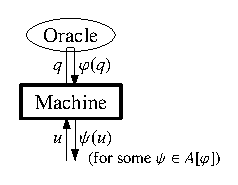
\includegraphics[scale=0.9]{./oracle_machine.eps}
\caption{A machine computing a multi-function $A \pcolon \LM \rightrightarrows \LM$.}
\label{figure: oracle machine}
\end{center}
\end{figure}

The \emph{size} of $\varphi \in \LM$, denoted $|\varphi|$,
is a (non-decreasing) function from $\N$ to $\N$ defined by 
$|\varphi|(|u|) = |\varphi(u)|$.
This is well-defined since a length-monotone function maps 
strings of the same length to strings of the same length.
To define the class $\classFPtwo$ of 
multi-functions from $\LM$ to $\LM$ 
computable in polynomial time, 
we bound the running time by \emph{second-order polynomials} 
$P (\lvert \varphi \rvert) (\lvert x \rvert)$ 
in the sizes of the oracle $\varphi$ and string $x$
given to the machine. 
A second-order polynomial $P (L) (n)$ 
is an expression built from the number $n$ 
using $\mathord+$, $\mathord\times$, 
\emph{and application of the function $L \colon \N \to \N$}; 
for example, 
$5 L (L (n) ^3 + n^2) + 2 n + 4$. 

\begin{definition}
 We write $\classFPtwo$ for the class of
 multi-functions from $\LM$ to $\LM$ 
 computed by a machine that runs
 in second-order polynomial time.
\end{definition}

We use bold letters (such as $\classFPtwo$) 
for classes of multi-functions from $\LM$ to $\LM$, 
as opposed to the usual complexity classes, such as $\classFP$, 
which we regard as consisting of multi-functions from $\varSigma ^*$ to $\varSigma ^*$.
The following is immediate. 

\begin{lemma}
\label{lemma: classFPtwo maps classFP to classFP}
 Functions in $\classFPtwo$ map 
 elements of $\classFP \cap \LM$ into $\classFP$.
\end{lemma}

For $\varphi$, $\psi \in \LM$, 
we define $\langle \varphi, \psi \rangle \in \LM$ by 
% \footnote{%
% The pairing function was
% defined erroneously in \cite{kawamura2012complexity} 
% without the delimiter $1$. 
% }
$\langle \varphi, \psi \rangle(0u) = \varphi(u) 10^{|\psi(u)|}$ and 
$\langle \varphi, \psi \rangle(1u) = \psi(u) 10^{|\varphi(u)|}$
(we pad $0$s to make $\langle \varphi, \psi \rangle$ length-monotone).
We write $\langle \varphi, \psi, \theta \rangle$ 
for $\langle \varphi, \langle \psi, \theta \rangle \rangle$, and so on.
We also write $\langle \varphi, u \rangle$, etc., for 
$\varphi \in \LM$ and a string $u \in \varSigma ^*$, 
by identifying $u$ with the constant function in $\LM$ with value $u$. 

\subsection{Representations}
\label{subsection: representations}

A \emph{representation} of a set $X$ 
is a partial function $\gamma$ from $\LM$ to $X$
such that for every $x \in X$ there is $\varphi$ with $\gamma (\varphi) = x$.
We call $\varphi$ a {\em $\gamma$-name} of $x$
if $x = \gamma (\varphi)$.

\begin{definition}
\label{definition: computation wrt representation}
\begin{enumerate}
\item 
Let $C$ be a class of multi-functions from $\varSigma ^*$ to $\varSigma ^*$, 
and let $\gamma$ be a representation of a set $X$. 
We write \emph{$\gamma$-$C$} for the set of $x \in X$
that have a $\gamma$-name in $C$.
\item  \label{enumi: computing wrt representation}
Let $\mathcal C$ be a class of multi-functions from $\LM$ to $\LM$,
and $\gamma$ and $\delta$ be representations of sets $X$ and $Y$, respectively.
A multi-function $A \pcolon X \rightrightarrows Y$
is in $(\gamma, \delta)$-$\mathcal C$ if 
the following multi-function $
\delta^{-1} \circ A \circ \gamma \pcolon \LM \rightrightarrows \LM
$ is in $\mathcal C$ (Figure~\ref{figure: realization}): 
\begin{figure}[t]
\begin{equation*}
  \xymatrix@C=50pt@R=16pt{
   \LM \ar[r] \ar[d] _\gamma & \LM \ar[d] ^\delta  \\
   X \ar[r] _A & Y 
  }
\end{equation*}
 \caption{$(\gamma, \delta)$-computing a multi-function~$A$.}
 \label{figure: realization}
\end{figure}
\begin{equation}
 (\delta^{-1} \circ A \circ \gamma)[\varphi] = 
  \begin{cases}
   \rlap{$\{\, \psi \in \dom \delta \mid \delta(\psi) \in A[\gamma(\varphi)] \,\}$} \hspace*{6em}
   \\
   & 
   \text{if } \varphi \in \dom \gamma, 
   \\ 
   \emptyset 
   &
   \text{otherwise.}
  \end{cases}
\end{equation}
\end{enumerate}
\end{definition}

For real numbers and real functions,
we use representations $\rhoR$ and $\deltabox$, 
defined as follows \cite{kawamura2012complexity}. 
We first introduce an encoding of dyadic numbers.
For each $n \in \N$, let $\D_n$ denote the set of strings of the form
\begin{equation}
 sx/1\!\underbrace{00\dots0}_{n},
\end{equation}
where $s$ is the sign and $x \in \{0,1\}^*$.
We write $\D$ for the union $\bigcup _n \D _n$.
We regard $u \in \D$ as a fraction of binary integers, 
and write $u$ also for the number it encodes. 

We define the representation~$\rhoR$ of $\R$ as follows: 
$\varphi \in \LM$ is a $\rhoR$-name of $x \in \R$ 
if $\varphi(0^i) \in \D$ and $\lvert \varphi(0^i) - x \rvert \le 2^{-i}$
for all $i \in \N$.
We write $\rhoR|^{[0,1]}$ for the representation of the interval $[0, 1]$ 
obtained by restricting $\rhoR$.
The class $(\rhoR|^{[0,1]},\rhoR)$-$\classFPtwo$ 
coincides with 
the polynomial-time computable functions by Ko~\cite{ko1991complexity}. 

We call $\mu \colon \N \to \N$ a {\em modulus of continuity} 
of $f \in \classC [0, 1]$ 
if 
for all $n \in \N$ and $x$, $y \in [0,1]$ with
$|x - y| \le 2^{-\mu(n)}$, 
we have $|f(x) - f(y)| \le 2^{-n}$ (Figure~\ref{figure: moc}). 
It is not hard to verify the following. 

\begin{lemma}
 \label{lem:type1representation}
 A real function $f \colon [0, 1] \to \R$ 
 is in $(\rhoR|^{[0,1]},\rhoR)$-$\classFPtwo$ if and only if
 it has a polynomial modulus of continuity 
 and there is a function $\varphi \in \classFP$ such that 
 \begin{equation}
   \label{eq:computation on rational points}
  |\varphi(d, 0^n) - f(d)| \le 2^{-n} 
 \end{equation}
 for all $d \in \D \cap [0,1]$ and $n \in \N$. 
\end{lemma}

The following representation $\deltabox$ of $\classC[0,1]$ 
is inspired by this. 
For a non-decreasing function $\mu \colon \N \to \N$, 
we write $\overline \mu \in \LM$ for the 
function that maps each string $u$ to $0^{\mu(|u|)}$.
A $\deltabox$-name of $f \in \classC[0,1]$ is 
a pair $\langle \overline{\mu}, \varphi \rangle$
(encoded in the way explained at the end of Section~\ref{section:TTF})
of $\varphi \in \LM$ and $\mu \colon \N \to \N$
such that 
$\mu$ is a modulus of continuity of $f$
and $\varphi$ satisfies \eqref{eq:computation on rational points}.
Lemma~\ref{lem:type1representation} implies that
$(\rhoR|^{[0,1]},\rhoR)$-$\classFPtwo$ equals
$\deltabox$-$\classFP$. 

\section{Small type-two classes}
\label{section:small-classes}

In this section, we introduce type-two complexity classes
corresponding to log-space $\classL$ and circuit complexity $\classNC$
based on the framework we reviewed in the previous section.
\begin{figure}
\begin{center}
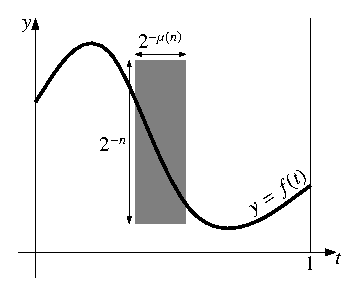
\includegraphics[scale=0.9]{./moc.eps}
\caption{Modulus of continuity~$\mu$ of a real function $f \in \classC [0, 1]$.}
\label{figure: moc}
\end{center}
\end{figure}
We also define $\classP$-completeness under log-space reductions.

\subsection{Logarithmic space}
\label{subsection: logspace}

As reviewed in the previous section, 
we use oracle Turing machines in the definition of type-two classes 
such as $\classFPtwo$. 
The machine has an input tape, output tape, work tape, query tape and answer tape. 
When the machine enters the query state, 
and the string on the query tape at that time is $u$, 
then in the next transition, 
the machine will be in the after-query state, and 
the string on the answer tape will be $\varphi (u)$, 
where $\varphi$ is the oracle
(although this exact mechanism for oracle access did not matter very much
for $\classFPtwo$ and larger classes). 
For the definition of 
the logarithmic-space class $\classFLtwo$, 
we will basically continue using this model, 
with space bound $\log (P (\lvert \varphi \rvert) (\lvert u \rvert))$
for the computation on oracle $\varphi$ and string input~$u$. 
To make this sub-linear space restriction meaningful, 
the standard convention (already for the type-one class $\classFL$) is that 
the input and output tapes are not counted towards the space limit, and that 
(to avoid exploiting these tapes as memory) 
the input tape is read-only and the output tape is write-only. 
For our purpose of type-two computation, 
we need to have similar consideration for query and answer tapes, 
and this raises some issues we should be careful about. 
(See also the discussion in the slightly different context of relativized classes 
\cite{aehlig2007relativizing,buss1988relativized,ladner1976relativization,wilson1988measure}.)

Note that even in this logarithmic-space setting, 
we want the machine to be able to ask queries of polynomial length. 
For example, when computing a real function $f$ under the $\rhoR$ representation, 
it is reasonable to give the machine access to 
the input real number with polynomially many digits of precision 
(in the number of digits we want of the output)---%
with logarithically many digits, 
we would only compute constant functions. 

Thus, the right formulation of logarithmic-space computation with oracle access 
requires careful resource control, by which 
the mechanism for oracle access is exempted from the space limit, 
while ``other parts'' of computation are limited to logarithmic space. 
For some special cases, 
this is achieved by simply adopting the convention that 
the query and answer tapes 
are not counted towards the space. 
In fact, Ko's logarithmic-space computable real functions on $[0, 1]$~%
\cite[Chapter~4]{ko1991complexity} is defined roughly in this way
(see the discussion in \cite[pp.~121--122]{ko1991complexity}), 
using a representation similar to our $\rhoR$. 
We also obtain the equivalent definition 
by the infinite string model, 
because it does not count the input and output tapes, 
and it forbids reading from the output tape. 

The reason this definition successfully led to a reasonable class of real functions
seems to be because, 
when we were dealing only with $\rhoR$-names, 
the queries were always of the simple form $0 ^m$. 
But in general, 
the queries are polynomially long binary string, 
which the machine cannot even store by itself on the work tape. 
This subtlety calls for the following modifications on the model
(as we will explain below): 

\begin{quote}
Our model is an oracle Turing machine 
with a stack of query tapes (write-only) and an answer tape (read-only).
The machine can write a symbol on the top query tape, or 
\emph{push} a new query tape on the top of the stack (and start writing on it).
When the machine issues a query, the stack is \emph{popped} automatically; 
that is, 
if the string on the query tape at the top of the stack was $u$, 
the oracle $\varphi$ writes the string $\varphi (u)$ on the answer tape, 
and at the same time the top query tape is removed from the stack. 
We put the restriction that the height of the stack of a machine is 
bounded by some constant for all inputs and oracles.
We also assume that 
the answer tape is erased after each push operation.
\end{quote}

This model resolves two issues that arise 
from the aforementioned tension between 
allowing the machine to issue long queries
while disallowing it to write them down. 

The first issue is that 
the machine may need to make nested queries 
(queries depending on answers to previous queries), and 
it may need to do so by writing a query halfway 
and then issuing other queries in order to complete the remaining part of the query.  
Observe that the stack model above makes such queries possible. 
The ability to ask nested queries (with constant depth of nesting) is needed naturally 
for our applications in real-number computation
(see e.g.\ the comments on Theorem~\ref{theorem:apply-is-L-computable} below), 
and is also essential if we want the class to contain
$\classFACtwo ^0$ 
(see Theorem~\ref{theorem:inclusion} below). 
The idea of using a stack of query tapes 
in order to obtain a reasonable relativization of logspace computation
is due to Wilson \cite{wilson1988measure} and 
Aehlig, Cook and Nguyen \cite{aehlig2007relativizing}
(but note that these are about predicate oracles). 
%% We choose this model because it is consistent with relativized circuit complexity classes.

The second issue (which arises because we are dealing with function oracles) is that 
we do not want the machine to cheat by 
using the query and answer tapes as extra memory. 
This is why we required that 
the answer tape is erased after each push operation. 
This makes our model equivalent to 
accessing the oracle $\varphi$ by questions of the form $(u, 0 ^i)$ 
asking for the $i$th bit of $\varphi (u)$ (or an explicit error message 
when $i$ exceeds the length of $\varphi (u)$).
The erasure of the answer tape also
ensures that the nested depth of queries is restricted to a constant.
Without this restriction, a log-space constant-stack machine with 
a function oracle $\varphi$ with $|\varphi|(n) = n$ 
could compute the result of iterating the function $\varphi$ polynomially many times.
On the other hand, there is a function $\varphi \in \LM$ such that $|\varphi|(n) = n$
and iteration of $\varphi$ is not in $\classNC$ relative to $\varphi$ \cite{aehlig2007relativizing}, 
and hence the inclusion $\classL \subseteq \classNC$ would not relativize.

\begin{definition}
 A machine (with the oracle access convention described above) 
 runs in (second-order) \emph{logarithmic space}
 if there is a second-order polynomial $P$ such that, 
 given oracle $\varphi \in \LM$ and string $u \in \varSigma^*$, 
 it visits at most $\log(P(|\varphi|)(|u|))$ cells
 in the work tape.
 We write $\classFLtwo$ for the set of multi-functions%
\footnote{%
We can of course define a class $\classLtwo$, 
analogous to $\classPtwo$ in \cite{kawamura2012complexity}, 
of multi-functions in $\classFLtwo$ whose values are functions in $\LM$ 
that are $\{0, 1\}$-valued, 
but we will not use such classes in this paper. 
}
 from $\LM$ to $\LM$ 
 computed by such a machine.
\end{definition}

\begin{lemma}
\label{lemma:Ltwo-maps-L-to-L}
 Functions in $\classFLtwo$ map 
 elements of $\classFL \cap \LM$
 into $\classFL$.
\end{lemma}

% \begin{proof}
% For all $\varphi \in \classFL$, the size of $\varphi$ is bounded by some polynomial,
% hence second-order logarithm collapses to first-order logarithm.
% Since $\classFL$ is low for itself ($\classFL^\classFL = \classFL$), 
% functions computed by log-space constant-stack machines with $\classFL$ oracle are in $\classFL$.
% \end{proof}

\subsection{Circuits of bounded depth}

In this section, we discuss the type-two analogue of $\classAC ^d$ and $\classNC$ 
by considering circuits with oracle gates.
Since the oracle in our setting has variable (second-order) sizes, 
and the resource (circuit size and depth) 
depends (second-order) polynomially on their size, 
the circuit family will be 
indexed not only by the size of the input string
but also by the size of the oracle. 
We will also see that the circuit classes are 
in the right containment with the 
Turing machine-based classes $\classLtwo$ and $\classPtwo$
from the previous sections. 

Let $n, m \in \N$ and let $L \colon \N \to \N$ be a non-decreasing function.
A \emph{circuit with size-$L$ oracle gates} is a circuit~$C$ 
(with several inputs and several outputs)
built from
the standard logical gates $\NOT$, $\OR$, $\AND$ (the latter two with unbounded fan-in) 
and oracle gates, 
where each oracle gate with $k$ inputs has $L (k)$ outputs.
The \emph{size} of $C$ is the number of gates.
The \emph{depth} of $C$ is the length of the longest path in $C$.
For an input $x \in \{0, 1\} ^*$, an oracle $\varphi \in \LM$, 
and a $|x|$-input $m$-output circuit $C$ with size-$|\varphi|$ oracle gates, 
we write $C^\varphi(x)$ for the $m$-bit output of $C$.

As mentioned above,
we consider \emph{oracle circuit families} $C = (C_{L,n})_{L,n}$, 
indexed by $n \in \N$ and non-decreasing functions $L \colon \N \to \N$,
such that each $C_{L, n}$ is an $n$-input circuit with size-$L$ oracle gates.
Such a family $C$ is said to
\emph{compute} a multi-function\footnote{%
As mentioned at the end of Section~\ref{section: introduction}, 
the family $C$ actually specifies a (single-valued) function, 
and thus the computed multi-functions are 
exactly those that underspecify this function. 
Nevertheless, we find it convenient to 
allow multi-functions in this definition, 
when we use it in combination with e.g.\ 
Definition~\ref{definition: computation wrt representation}.\ref{enumi: computing wrt representation}.
}
$A \pcolon \LM \rightrightarrows \LM$ if 
for all $\varphi \in \dom A$, there is $\psi \in A[\varphi]$ 
satisfying $\psi(x) = C_{|\varphi|, |x|}^\varphi(x)$ for all $x \in \varSigma^*$.

This family $(C_{L,n})_{L,n}$ is said to have
\emph{polynomial size} 
if there is a second-order polynomial $P$ such that 
the size of $C _{L,n}$ is bounded by $P (L) (n)$. 
Likewise, it has \emph{$k$-logarithmic depth}
if there is a second-order polynomial $P$ such that 
each $C _{L,n}$ has depth bounded by $(\log (P(L)(n))) ^k$. 

\begin{figure*}
\begin{center}
\hfill
\parbox[t]{150pt}{\centering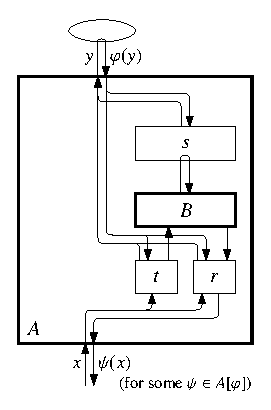
\includegraphics[scale=0.9]{./redtwom.eps}\\[3pt]$A \redLmF B$}
\hfill
\parbox[t]{150pt}{\centering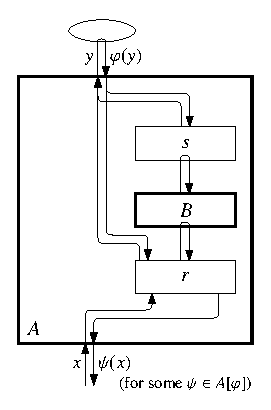
\includegraphics[scale=0.9]{./redtwoT.eps}\\[3pt]$A \redLW B$}
\hfill
\parbox[t]{150pt}{\centering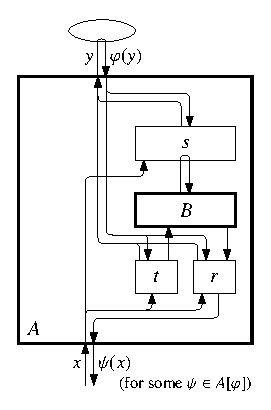
\includegraphics[scale=0.9]{./redtwoBCEIP.eps}\\[3pt]$A \redLB B$}
\hfill\mbox{}
\caption{Reductions between multi-functions on $\LM$.}
\label{figure: intermediate many-one reduction}
\end{center}
\end{figure*}

The definition of uniformity 
also takes into account the oracle size: 
we say that the family $(C_{L,n})_{L,n}$ is 
\emph{$\classLtwo$-uniform} if 
there is a function $A \in \classFLtwo$ such that 
for all $n \in \N$ and non-decreasing $L \colon \N \to \N$, 
the string $A (\overline L) (0^n)$ is (a description of) the circuit $C_{L,n}$ 
(recall from the end of Section~\ref{subsection: representations} 
that $\overline L$ is the function taking strings $u$ to $0 ^{L (\lvert u \rvert)}$). 
Hereafter, we assume log-space uniformity on all (type-one and type-two) 
circuit classes, so we write just ``uniform'' or omit ``$\classLtwo$-uniform''.

\begin{definition}
 For each $k \in \N$, 
 we write $\classFACtwo^k$ for the class of 
 multi-functions from $\LM$ to $\LM$ computed by
 a (uniform) circuit family $(C_{L,n})_{L,n}$ 
of polynomial size and $k$-logarithmic depth%
\footnote{We are thus defining the analogue of $\classNC$ as the union of 
$\classAC^i$ rather than of $\classNC^i$.  This is just for simplicity of presentation.}. 
 We write $\classFNCtwo = \bigcup_{k \in \N} \classFACtwo^k$.
\end{definition}

Similarly to the type-one class $\classFP$, it is easy to see that
a multi-function $A \pcolon \LM \rightrightarrows \LM$ is computed by a polynomial-size
uniform circuit family if and only if $A \in \classFPtwo$
(for the ``if'' part, we modify the standard argument for the type-one class, 
noting that any $A \in \classFPtwo$ can be computed by 
an ``oblivious'' polynomial-time machine 
whose head motions depend only on the sizes of 
the input string and the oracle).

The relativization using the stack model by Aehlig, Cook and Nguyen preserves
the inclusion of non-relativized classes
$\classAC^0 \subseteq \classL \subseteq \classAC^1 \subseteq \classNC$.
Since we define the type-two log-space class by extending the stack model,
the analogous inclusions can be shown for our type-two classes
by a similar argument. 

\begin{theorem}
\label{theorem:inclusion}
$ \classFACtwo^0
 \subseteq \classFLtwo 
 \subseteq \classFACtwo^1
 \subseteq \classFNCtwo
 \subseteq \classFPtwo$. 
\end{theorem}

\begin{proof}
 The first inclusion can be proved similarly
 to $\classAC^0 \subseteq \classL$ (thanks to the stack model, as we mentioned 
 in Section~\ref{subsection: logspace}).
 The second inclusion can be proved by an argument similar to
 $\text{cs}\classL(\alpha) \subseteq \classAC^1(\alpha)$
 \cite{aehlig2007relativizing}.
 The third inclusion is immediate.
 The last inclusion follows from the above characterization of $\classFPtwo$
 by $\classLtwo$-uniform families of polynomial-size circuits.
\end{proof}

The following lemma states that $\classLtwo$-uniformity respects
$\classL$-uniformity.

\begin{lemma}
\label{lemma: respects uniformity}
 Let $C = (C _{L, n}) _{L, n}$ be a 
 polynomial-size $\classLtwo$-uniform oracle circuit family, 
 and $D = (D _n) _n$ be a (usual) polynomial-size $\classL$-uniform circuit family.
 Let $L _D (n)$ denote the output size of the circuit $D _n$, 
 and let $C _{L _D, n} ^D$ be 
 defined by replacing each oracle gate in $C _{L _D, n}$
 by the circuit (with the appropriate input size) from $D$. 
 Then the circuit family $C ^D := (C _{L _D, n} ^D) _n$ is $\classL$-uniform.
\end{lemma}

\begin{proof}
 Let $A \in \classFLtwo$ be a function 
 describing $C$ (as in the above definition of $\classLtwo$-uniformity), 
 and 
 $B \in \classFL$ be a function 
 describing $D$.
 Since $\overline{L _D} \in \classFL$ and $A \in \classFLtwo$, 
 we have $A(\overline{L _D}) \in \classFL$. 
 Since the description of $C ^D$ can be computed in log-space
 given $A(\overline{L _D})$ and $B$ as oracles, 
 it is in $\classFL$. 
\end{proof}

\begin{lemma}
\label{lemma: type-one and type-two circuit classes}
\begin{enumerate}
 \item Functions in $\classFACtwo^i$ 
       map elements of $\classFAC^j \cap \LM$ 
       into $\classFAC^{i+j}$.
 \item Functions in $\classFNCtwo$
       map elements of $\classFNC \cap \LM$ 
       into $\classFNC$.
\end{enumerate}
\end{lemma}

\begin{proof}
We prove the first part (the second part follows immediately).
Let $A$ be a function in $\classFACtwo^i$ and $C = (C_{L,n})_{L,n}$ be an 
($i$-logarithmic depth) oracle circuit family computing $A$. 
For all $\varphi \in \classFAC^j \cap \LM$, 
the circuit family $C ^\varphi$ is 
of (first-order) polynomial size and its depth is $i$-logarithmic,
since there is a polynomial $p$ satisfying $|\varphi|(n) \le p(n)$.
Let $(D_n)_n$ be a circuit family of depth $O(\log^j(n))$
computing $\varphi$.
Replacing oracle gates in $(C^\varphi_n)_n$ by $(D_n)_n$, 
we get a circuit family with polynomial size and $\log^{i+j}(n)$ depth
that computes $A(\varphi)$.
\end{proof}

\subsection{Reductions and completeness}

The formulation of reduction and hardness 
is mostly analogous to what was done for larger classes 
already in \cite{kawamura2012complexity}, 
simply using weaker (logspace) reduction this time. 
We will present the definitions for the sake of completeness. 
The following logspace reductions $\redLmF$, $\redLW$, $\redLB$
(Figure~\ref{figure: intermediate many-one reduction}) are
analogues of the polynomial-time reductions 
$\redmF^2$, $\redW^2$ in Kawamura and Cook~\cite{kawamura2012complexity}
and the ``many-one reduction'' in Beame et al.~\cite{beame1995relative}. 

\begin{definition}
Let $A$, $B \pcolon \LM \rightrightarrows \LM$ be multi-functions.
\begin{itemize}
 \item $A$ is \emph{many-one log-space reducible} to $B$, 
       denoted $A \redLmF B$,
       if there are functions $r, s, t \in \classFLtwo$ such that 
       for all $\varphi \in \dom A$,
       we have $s(\varphi) \in \dom B$ and 
       for each $\theta \in B[s(\varphi)]$, 
       the function that maps $x \in \varSigma^*$ to $r(\varphi)(x, \theta(t(\varphi)(x)))$
       is in $A[\varphi]$.
 \item $A$ is \emph{Weihrauch log-space reducible} to $B$,
       denoted $A \redLW B$,
       if there are functions $r, s \in \classFLtwo$ such that 
       for all $\varphi \in \dom A$,
       we have $s(\varphi) \in \dom B$ and 
       for each $\theta \in B[s(\varphi)]$, 
       we have $r(\langle \varphi, \theta \rangle) \in A[\varphi]$.
 \item $A \redLB B$ 
if there are functions $r, s, t \in \classFLtwo$ such that 
for all $\varphi \in \dom A$,
the function~$\sigma$ that maps $y \in \varSigma ^*$ to $s (\varphi) (x, y)$
belongs to $\dom B$ 
and for each $\theta \in B [\sigma]$, 
the function that maps $x \in \varSigma^*$ 
to $r(\varphi)(x, \theta(t(\varphi)(x)))$ is in $A[\varphi]$.
\end{itemize}
\end{definition}

For a class $\mathcal{C}$ of multi-functions from $\LM$ to $\LM$
and a reduction $\leq$, 
we say that $B \pcolon \LM \rightrightarrows \LM$ is 
\emph{$\mathcal{C}$-$\leq$-hard} if $A \leq B$ for all $A \in \mathcal{C}$,
and $B$ is \emph{$\mathcal{C}$-$\leq$-complete} 
if $B$ is $\mathcal{C}$-$\leq$-hard and in $\mathcal{C}$.

Note that $A \redLmF B$ implies $A \redLW B$ and $A \redLB B$. 
The reduction $\redLB$ is stronger than $\redLmF$ in that 
$s$ can read the input string $x$ when answering queries from $B$.
In many applications to analysis, 
the (thus easier) proof of $\redLB$-hardness 
already seems to capture the essential complexity of the operator
(e.g.~Theorem~\ref{theorem:P-hard-g_u} in our case), 
but we need the stronger hardness (with $\redLmF$ or $\redLW$)
if we want to derive the non-uniform versions just from the statement
(see the next lemma, which does not hold for
$\redLB$; cf.~\cite[Lemma~3.6]{kawamura2012complexity}). 

For $F \subseteq \LM$, 
define the multi-function $\bigcup F \pcolon \varSigma ^* \rightrightarrows \varSigma ^*$ by
$(\bigcup F) [x] = \{\, f(x) \mid f \in F \,\}$.
The following lemma (see appendix for a proof)
will help us in Section~\ref{section:P-complete} to show that 
our uniform statements ($\classFPtwo$-$\redLmF$-hardness of an operation)
imply the known non-uniform results 
\newcommand{\redoneLmF}{\le^\classL_{\mathrm{mF}}}
(existence of an $\classFP$-$\redoneLmF$-hard output, 
where $\redoneLmF$ is the usual many-one log-space reduction 
between type-one multi-functions.). 

\begin{lemma}
\label{lemma:P-complete}
If $B \pcolon \LM \rightrightarrows \LM$ is $\classFPtwo$-$\redLmF$-complete, 
there is $\psi \in \dom B \cap \classFL$ such that
 $\bigcup (B[\psi])$ is $\classFP$-$\redoneLmF$-complete. 
\end{lemma}

\begin{proof}
Let $A \colon \LM \to \LM$ be a constant function 
whose value is 
an $\classFP$-$\redoneLmF$-complete function. 
% (such as the \emph{circuit value problem}).
Note that $A \in \classFPtwo$.
Let $r$, $s$, $t \in \classFLtwo$ be functions that reduce $A$ to $B$
as in the definition of $\redLmF$.
Choose any $\varphi \in \classFL$, 
and it follows from Lemma~\ref{lemma:Ltwo-maps-L-to-L}
that $r(\varphi)$, $s(\varphi)$, $t(\varphi) \in \classFL$.
Let $\psi = s(\varphi)$, then $r (\varphi)$ and $t (\varphi)$ 
give the reduction 
$A (\varphi) \redmF^\classL \bigcup (B[\psi])$.
Since $A(\varphi)$ is $\classFP$-$\redmF^\classL$-complete,
so is $\bigcup (B[\psi])$.
\end{proof}

The following partial function $\probDTIMEtwo \pcolon \LM \to \LM$ 
is a standard complete problem: 
$\dom \probDTIMEtwo$ consists of $\langle M, \overline \mu, \varphi \rangle$
such that $M$ is (the program of) a machine, 
$\mu \colon \N \to \N$ is non-decreasing, 
$\varphi \in \LM$, 
and $M^\varphi(x)$ stops in $\mu(|x|)$ steps for all $x \in \varSigma^*$; 
for such $\langle M, \overline \mu, \varphi \rangle$, 
we define $\probDTIMEtwo(\langle M, \overline \mu, \varphi \rangle)(x)$ to be 
the output of the computation $M^\varphi(x)$.

\begin{lemma}
\label{lemma: probDTIMEtwo}
 $\probDTIMEtwo$ is $\classFPtwo$-$\redLmF$-complete.
\end{lemma}

\begin{proof}
 Let $A \in \classFPtwo$. 
 There is a machine $M$ computing $A$
 in time bounded by a second-order polynomial $P$. 
 Then $r (\varphi) (u, \probDTIMEtwo(s(\varphi))(t(\varphi)(u))) = M ^\varphi (u) = A (\varphi) (u)$, 
 where 
 $r$, $s$, $t \in \classFLtwo$ are given by 
 $r (\varphi) (u, v) = v$, 
 $s (\varphi) = \langle M, \overline{P(\mu)}, \varphi \rangle$ and 
 $t (\varphi) (u) = u$.
\end{proof}

% We define a partial function  $\probCVPtwo \pcolon \LM \to \LM$ as follows:
% $\dom \probCVPtwo$ is the set of $\langle (C_n)_n, \varphi \rangle$
% such that $C_n$ is (the description of) a circuit with $n$ inputs 
% (and multiple outputs)
% consisting of $\AND$, $\OR$, $\NOT$ and oracle gates, 
% for which $\varphi \in \LM$ has the right size.
% For $\probCVPtwo(\langle (C_n)_n, \varphi \rangle)(x) = C^\varphi_{|x|}(x)$.

% \begin{lemma}
%  $\probCVPtwo$ is $\classFPtwo$-$\redLmF$-complete.
% \end{lemma}

% \begin{proof}
% Similar to Theorem~\ref{theorem:P-equals-L-uniform-P-poly}.
% \end{proof}

\subsection{Representations}
\newcommand{\transL}{\preceq_\classLtwo}

Carrying over the above arguments to represented spaces
is also analogous to what has been done \cite{kawamura2012complexity} for larger classes. 
Let $\gamma$ and $\delta$ be representations of $X$ and $Y$, respectively.
Definition~\ref{definition: computation wrt representation} 
tells us when 
a point $x \in X$ is in $\gamma$-$\classFL$ or $\gamma$-$\classFNC$, 
and when a multi-function $A \pcolon X \rightrightarrows Y$ is in
$(\gamma, \delta)$-$\classFLtwo$ or
$(\gamma, \delta)$-$\classFNCtwo$. 
We also define hardness under representations: 
$x$ is $\gamma$-$C$-$\le$-\emph{hard} if
$\bigcup(\gamma^{-1}[x])$ is $C$-$\le$-hard,
where $\gamma^{-1}[x]$ is the set of $\gamma$-names of $x$; 
and $A$ is $(\gamma, \delta)$-$\classFPtwo$-$\le$-\emph{hard}
if $\delta^{-1} \circ A \circ \gamma$ 
(see Definition~\ref{definition: computation wrt representation}) 
is $\classFPtwo$-$\le$-hard.
The following facts
about translation between representations are
analogous to \cite{kawamura2012complexity}. 

\begin{definition}
Let $\gamma$ and $\delta$ be two representations of a set $X$.
We write $\gamma \transL \delta$ if
there is a function $F \in \classFLtwo$ \emph{translating} $\gamma$-names
into $\delta$-names, that is, 
$F (\varphi) \in \dom \delta$ and $\delta(F(\varphi)) = \gamma (\varphi)$ 
for all $\varphi \in \dom \gamma$.
\end{definition}

\begin{lemma}
 Let $\gamma$ and $\gamma'$ be representations of a set $X$, 
 $\delta$ and $\delta'$ be representations of a set $Y$.
 If $\gamma \transL \gamma'$ and $\delta \transL \delta'$, then 
\begin{enumerate}
\item 
$(\gamma', \delta)$-$\mathcal C \subseteq (\gamma, \delta')$-$\mathcal C$, 
for $\mathcal{C} = \classFLtwo$, $\classFNCtwo$ or $\classFPtwo$; 
\item 
a $(\gamma, \delta')$-$\classFPtwo$-$\redLW$-hard multi-function is
$(\gamma', \delta)$-$\classFPtwo$-$\redLW$-hard.
\end{enumerate}
\end{lemma}

Although this shows that $\redLW$-hardness is 
more stable and perhaps natural 
than $\redLmF$-hardness, 
we will state some of our hardness results in Section~\ref{section:applications}
using $\redLmF$, 
simply in the interest of proving stronger statements
(and deriving the existing non-uniform counterparts as corollaries
through the following lemma). 

The following lemma is the version of 
Lemmas~\ref{lemma: classFPtwo maps classFP to classFP}, 
\ref{lemma:Ltwo-maps-L-to-L}, 
\ref{lemma: type-one and type-two circuit classes} and 
\ref{lemma:P-complete} for represented spaces, 
and follows easily from them. 

\begin{lemma}
\label{lemma:p-comp-maps-l-to-p-comp}
 Let $\gamma$ and $\delta$ be representations of sets $X$ and $Y$, respectively.
\begin{enumerate}
\item
 A partial function in $(\gamma, \delta)$-$\mathcal C$
 maps all elements of $\gamma$-$C$ in its domain into $\delta$-$C$, 
 where $\mathcal C$ is $\classFLtwo$, $\classFNCtwo$, or $\classFPtwo$ 
 and $C$ is the corresponding type-one class. 
\item \label{enumi:p-comp-maps-l-to-p-comp}
 A $(\gamma, \delta)$-$\classFPtwo$-$\redLmF$-complete partial function 
 maps some element of $\gamma$-$\classFL$ 
 to a $\delta$-$\classFP$-$\redmF^\classL$-complete element of $Y$.
\end{enumerate}
\end{lemma}

\section{Applications}
\label{section:applications}

In Section~\ref{section:function}, 
we show some examples of real functions and operators 
that are in $\classFLtwo$ and $\classFNCtwo$ (under suitable representations). 
In Section~\ref{section:P-complete}, we show the $\classPtwo$-completeness of 
the inverse operation and the fix-point operation.

\subsection{Within $\classFLtwo$ and $\classFNCtwo$}
\label{section:function}

We start with real numbers and real functions, 
using the representation $\rhoR$
(see Section~\ref{subsection: representations}). 
Ko's class of
\emph{log-space real functions} in $\classC[0,1]$ 
\cite{ko1991complexity} 
coincides with our $(\rhoRunit, \rhoR)$-$\classFLtwo$, 
despite our choice of constant-stack log-space machine 
while Ko uses the obvious log-space oracle Turing machine 
with no stack.
This is because, 
when computing approximation of $f(x)$ under $\rhoR$-names, 
a machine can get enough information about $x \in [0,1]$ in one query
(recall from Section~\ref{subsection: logspace} that 
the reason we needed the stack model 
was to set the right convention for nested queries).

Ko also defines the class of $\classNC$ real functions in $\classC[0,1]$
as $\deltabox$-$\classFNC$ in our terminology 
\cite{ko1991complexity},
which easily equals $(\rhoRunit, \rhoR)$-$\classFNCtwo$.
The $\classNC$-real functions from $\R$ to $\R$ defined by Hoover \cite{hoover1991real}
are exactly those in $(\rhoR, \rhoR)$-$\classFNCtwo$.

An important update to our knowledge
after the publication of Ko's book~\cite{ko1991complexity} was the 
discovery by Chiu, Davida and Litow~\cite{chiu2001division}
of a logarithmic space algorithm 
for division and iterated multiplication. 
This is especially important in our context of computable analysis, 
because it enables us to evaluate a fast-converging Taylor series, 
by which many real numbers and functions are defined. 
Thanks to this, we can see 
in Examples \ref{example: pi} and \ref{example: sine}
that the considered functions are not just in $\classFNCtwo$ but also in $\classFLtwo$. 

For representations $\gamma _0$, $\gamma _1$ of 
spaces $X _0$, $X _1$, respectively, 
we define the representation $[\gamma _0, \gamma _1]$
of the Cartesian product $X _0 \times X _1$ by 
setting $
  [\gamma _0, \gamma _1] (\langle \varphi _0, \varphi _1 \rangle) 
= 
  (\gamma _0 (\varphi _0), \gamma _1 (\varphi _1))
$ for each $\varphi _0$, $\varphi _1 \in \LM$
(recall that $\langle \mathord\cdot, \mathord\cdot \rangle$
is the pairing function defined at the end of Section~\ref{section:TTF}). 

\begin{example}
 The binary addition and the binary multiplication are
 in $([\rhoR, \rhoR], \rhoR)$-$\classFLtwo$.
\end{example}

\begin{example}
\label{example: pi}
The circle ratio $\pi$ is in $\rhoR$-$\classFL$ because the series
\begin{equation}
 \pi = \sum_{k=0}^\infty \frac{1}{16^k} 
  \left( \frac{4}{8k+1} - \frac{2}{8k+4} - \frac{1}{8k+5} - \frac{1}{8k+6} \right)
\end{equation}
converges fast enough, 
so that a $2 ^{-n}$-approximation to $\pi$ can be obtained by adding up 
an appropriate number $k = \mathrm O (n)$ of terms. 
This computation of approximate partial sum involves 
polynomially many multiplications, additions, and divisions on rationals, 
and each of these operations can be performed in logarithmic space
by Chiu, Davida and Litow~\cite{chiu2001division}.
\end{example}

% \begin{lemma}
%  The exponential function restricted to $[0,1]$
%  is in $(\rhoRunit, \rhoR)$-$\classFLtwo$.
% \end{lemma}
% Since the series $\exp(t) = \sum_n x^n / n!$ converges fast enough,
% a $2^{-m}$-approximation of $\exp(t)$ for $t \in [0,1]$ can be computed
% by polynomially many multiplications, additions, and divisions on rationals. 

% On the other hand, without the restriction on the domain, $\exp$ is not 
% even in $(\rhoR, \rhoR)$-$\classFPtwo$, 
% because it grows too fast. 

\begin{example}
\label{example: sine}
The sine function $\sin \colon \R \to \R$ is
in $(\rhoR, \rhoR)$-$\classFLtwo$.
To see this, note that 
the Taylor series of $\sin$ also converge fast enough,
so it is log-space computable if restricted to $[-4, 4]$.
The multi-function that computes from $t$
any $x \in [-4, 4]$ with $x \equiv t \bmod 2 \pi$ is
in $(\rhoR, \rhoR|^{[-4,4]})$-$\classFLtwo$, 
because division is log-space computable 
and $\pi \in \rhoR$-$\classFL$. 
Combining these, $\sin \in (\rhoR, \rhoR)$-$\classFLtwo$.
\end{example}

The following states that $\deltabox$ 
is the weakest representation that makes function evaluation 
logspace computable, 
and gives evidence that 
$\deltabox$ is the natural choice (relative to $\rhoR$)
as a basic representation of $\classC [0, 1]$. 
It can be proved similarly to the analogous theorem for $\classFPtwo$ 
\cite{kawamura11:_funct_space_repres_and_polyn_time_comput}. 
Define $\OpApply \colon \classC [0, 1] \times [0, 1] \to \R$ by 
$\OpApply (f) (x) = f (x)$. 

\begin{theorem}
 \label{theorem:apply-is-L-computable}
 Let $\delta$ be a representation of $\classC[0, 1]$.
 $\OpApply$ is in $([\delta, \rhoRunit], \rhoR)$-$\classFLtwo$ if
 and only if $\delta \transL \deltabox$.
\end{theorem}

Note that, 
if we had defined $\classFLtwo$ with the obvious relativized machine with one query tape,
$\classFLtwo$ would be either too weak 
to have $\OpApply \in ([\deltabox,\rhoR], \rhoR)$-$\classFLtwo$ or
too strong to be a subset of $\classFNCtwo$,
depending on whether or not the machine is allowed to look at the answer tape while writing queries.
% Our extension of the constant stack model is the weakest
% such that both Theorem~\ref{theorem:apply-is-L-computable} and 
% $\classFLtwo \subseteq \classFNCtwo$ true.

In the rest of Section~\ref{section:function}, 
we reformulate in our terminology a known result that 
informally reads
``the roots of a complex polynomial can be found in $\classNC$.'' 

We write $P_n$ for the set of degree-$n$ monic 
polynomials (i.e.\ the leading coefficient is $1$) with complex coefficients.
We write $\OpPolyRoot(p)$ for the multiset of all the roots of $p \in P_n$, that is, $p(x) = \prod_{z \in \OpPolyRoot(p)} (x - z)$. 
Neff first showed the following theorem, which says that 
approximating the roots of polynomial
with integer (or rational, equivalently) coefficients is in $\classFNC$.
We write $|p|$ for the maximum absolute value of coefficients in $p$.

\begin{theorem}
[NC polynomial root isolation \cite{neff1994specified}]\label{theorem:neff1994}
There is an algorithm $A$ such that,
for any choice of integers $n$, $m$, $k$, and a polynomial $p \in P_n$
with $|p| \le 2^m$,
$A$ computes $k$-digit approximation to the roots of $p$ 
in at most $C \log^e(n + m + k)$ parallel steps, 
using at most $D(n + m + k)^f$ processors, where $C, D, e, f$ are positive
constants which are independent of $n$, $m$, and $k$.
\end{theorem}

Later Pan showed that approximating the roots of a polynomial
with complex rational coefficients is in $\classFNC$ \cite{pan1995optimal}.
Neff and Reif showed a similar result and they also discuss
the modulus of continuity of finding roots \cite{neff1996efficient}.

\begin{theorem}
[{\cite[Theorem 2.1]{neff1996efficient}}]
\label{neff1996modulus}
 Let $f$ and $g$ be monic polynomials of the same degree $n$,
 and let $|f| \le 2^m$.
 For each $k \in \N$, 
 if $|f - g| \le 2^{\lceil n(k + m + \log n + 3)\rceil}$, then
 $d(\OpPolyRoot(f), \OpPolyRoot(g)) \le 2^{-k}$. 
\end{theorem}

% They regard these two results ensure that $\classFNC$-computability
% of finding roots of a polynomial with complex coefficients.%%??????
% In our framework, we can combine these two results by stating 
% $\classFNCtwo$-computability under suitable representations.

These can be recast into our framework by specifying 
representations for polynomials and multisets of complex numbers as follows.
We represent a complex number by a pair of $\rhoR$-names,
i.e., $
 \rho_\C (\langle \varphi, \psi \rangle) 
= 
 \rhoR (\varphi) + \sqrt{-1} \cdot \rhoR (\psi)
$.  We define the representation $\rho_{P_n}$ of 
$P _n$ as follows: 
$\varphi = \langle \varphi _0, \ldots, \varphi _{n - 1} \rangle \in \LM$ 
is a $\rho_{P_n}$-name of $p \in P_n$ if 
$\varphi _0$, \ldots, $\varphi _{n - 1}$ are 
$\rho_{\C}$-names of $a _0$, \ldots, $a _{n - 1}$, respectively, 
with $p(x) = x^n + a_{n-1}x^{n-1} + \dots + a_0$.
Define the representation $\rho_{P_*}$ of all monic polynomials by
$\rho_{P_*}(\langle 0^n, \varphi \rangle) = \rho_{P_n}(\varphi)$.
Define the representation $\rhoCSet$ for finite multisets of complex numbers 
as follows:
$\varphi \in \LM$ is a $\rhoCSet$-name of a multiset $S$ if 
for each $m \in \N$, 
we have $\varphi(0 ^m) = ( a_1, b_1, a_2, b_2, \dots, a_n, b_n )$
with $a_1, b_1, \dots, a_n, b_n \in \D_m$
such that 
$d(S, \{a_1 + b_1 \sqrt{-1}, \dots, a_n + b_n \sqrt{-1}\}) \le 2^{-m}$, 
where the distance between two multisets is defined as $
 d (\{z_1, \dots, z_n\}, \{z'_1, \dots, z'_n\}) 
= 
 \min_{\sigma} \max_{j = 1, \ldots, n}|z_j - z'_{\sigma(j)}|
$, with $\sigma$ ranging over all permutations on $\{1, \ldots, n\}$. 

%We can also represent multisets $S$ as vectors $z \in \C^n$
%such that $S = \{z\}$.
%More formally we define representation $\rhoCSet'$ as
%$\rhoCSet'(\varphi) = \{z\}$ if $\rho_{\C^*}(\varphi) = (z_1, \dots, z_n)$.
%It is easy to see that $\rhoCSet' \le_\classFLtwo \rhoCSet$,
%but the following lemma says they are not equivalent even under computability.
%\begin{lemma}
% Identity function on multisets is not $(\rhoCSet, \rhoCSet')$-computable.
%\end{lemma}
%This means that $\rhoCSet'$ is more informative than $\rhoCSet$.
%\paragraph{Finding polynomial roots is $\classFNCtwo$-computable}

\begin{theorem}
 \label{theorem:finding-roots-is-in-NC}
 $\OpPolyRoot$ is in $(\rho_{P_*}, \rhoCSet)$-$\classFNCtwo$.
\end{theorem}

% \begin{corollary}
%  $\OpPolyRoot$ is $(\rho_{P_n}, \rhoCSet)$-$\classFNCtwo$-computable.
% \end{corollary}

\begin{proof}
This is immediate by the following algorithm
using the above-cited facts:
Given $k \in \N$ and a $\rho_{P_n}$-name of $p \in P_n$, 
compute a polynomial $q \in {P_n}$ with complex rational coefficients
satisfying $|p - q| \le 2^{\lceil n((k+1) + m + \log n + 3)\rceil}$.
By Theorem~\ref{neff1996modulus}, the difference between 
the roots of $p$ and $q$ is at most $2^{-(k+1)}$.
Output approximate roots of $q$ with precision $2^{-(k+1)}$ 
computed by the algorithm by Neff and Reif, or Pan,
which are $2^{-k}$-approximations of roots of $p$.
\end{proof}

\subsection{$\classPtwo$-complete operations}
\label{section:P-complete}

Here we state and prove uniform versions of 
Hoover's and Ko's $\classP$-hardness results 
about operators on real functions. 
As mentioned in the introduction, 
this is only possible with our type-two formulation of complexity classes. 

\enlargethispage{4pt}

\subsubsection{Inverting a function}

Fix $a$, $b \in \R$ with $a < b$. 
Let $M$ be the set of one-to-one functions $f \in \classC[0,1]$
whose range is $[a,b]$.
We define the function $\OpINV \colon M \to \classC [a, b]$ 
by saying that $\OpINV (f) = f ^{-1}$ is the inverse function of $f$. 

Ko proved the following non-uniform theorem about the complexity of inversion.
Recall that Ko's polynomial-time and log-space computability of a real function
is equivalent to our $(\rhoRunit, \rhoR)$-$\classFPtwo$ and $(\rhoRunit, \rhoR)$-$\classFLtwo$. 

\begin{theorem}
[{\cite[Corollary 4.7 and Theorem 4.18]{ko1991complexity}}]
\label{theorem: ko inversion}
\begin{enumerate}
\item \label{enumi:ko1991-4.7}
Assume that $f \in M$ is polynomial-time computable. 
If $f^{-1}$ has a polynomial modulus of continuity, 
then $f^{-1}$ is polynomial-time computable.
\item \label{enumi:ko1991-4.18}
There is a log-space computable $f \in M$
such that $f^{-1}$ has a polynomial modulus of continuity
but $f^{-1}$ is not log-space computable
unless $\classP = \classL$.
\end{enumerate}
\end{theorem}

We define a representation $\deltaboxINV$ of $M$ as follows:
$\deltaboxINV(\langle \varphi, \overline{\mu} \rangle) = f$ 
if and only if $\varphi$ is a $\deltabox$-name of $f$ 
and $\mu$ is a modulus of continuity of $f^{-1}$.
We add a modulus of continuity of $f^{-1}$ to $\deltabox$
since without this information, there is no upper bound on 
the complexity of the inverse operation, 
as the following fact \cite[Theorem 4.4]{ko1991complexity} shows: 
for any recursive $x \in [0, 1]$, 
there exists a strictly increasing function $f \in \classC[0, 1]$ 
such that $f$ is polynomial-time computable and $x = f^{-1}(0)$.

The following theorem is the uniform version of Theorem~\ref{theorem: ko inversion}. 
Part~\ref{enumi:ko1991-4.7} of Theorem~\ref{theorem: ko inversion} 
follows from this and Lemma~\ref{lemma: classFPtwo maps classFP to classFP}.
Part~\ref{enumi:ko1991-4.18} follows from this theorem and Lemma~\ref{lemma:p-comp-maps-l-to-p-comp}.\ref{enumi:p-comp-maps-l-to-p-comp}.

\begin{theorem}
 \label{theorem:INV-is-P-complete}
 $\OpINV$ is $(\deltaboxINV, \deltabox)$-$\classFPtwo$-$\redLmF$-complete.
\end{theorem}

This will be proved in the appendix, 
using 
Theorem~\ref{theorem:P-hard-g_u} below. 

\subsubsection{Fixed points of contractions}

A function $g \colon K \to \R$ on a set $K \subseteq \R$
is called $q$-\emph{Lipschitz}, for $q > 0$, 
if $
\lvert g (x) - g (y) \rvert \leq q \cdot \lvert x - y \rvert
$ for all $x$, $y \in K$. 
A \emph{contraction} on $K$ is 
a function $g \colon K \to \R$ which is $q$-Lipschitz for some $q < 1$
and whose values are in $K$. 
The Banach fixpoint theorem states that 
a contraction has a fixed point and it is unique. 
Hoover's theorem about the complexity of computing the fixed point
of a contraction can be written in our terminology as follows:

\begin{theorem}
[{\cite[Theorem 4.5]{hoover1991real}}]
\label{theorem:hoover1991-4.5}
 There is a function $f \colon \R \to \R$ in $(\rhoR, \rhoR)$-$\classFNCtwo$
 whose restriction $f|_{[2k, 2k+1]}$ is a contraction for each $k \in \N$ and
 which has the following property: 
 $\classNC = \classP$ if and only if 
 there is a function (from strings to strings) in $\classFNC$ mapping 
 a pair of a number $k \in \N$ (written in binary) and the string $0^n$
 to a $2^{-n}$-approximation of the 
 fixed point of $f |_{[2k, 2k + 1]}$. 
\end{theorem}

For our formulation in TTE, 
let $C$ be the set of contractions on $[0, 1]$. 
We define its representation $\deltaboxCM$ by saying that 
a \emph{$\deltaboxCM$-name} of $g \in C$
is a pair $\langle \varphi, q \rangle$ of 
a $\deltabox$-name $\varphi \in \LM$ of $g$ 
and a dyadic number $q \in \D$ such that $g$ is $q$-Lipschitz. 
Let $\OpCMFix \colon C \to \R$ be the function
taking each contraction on $[0, 1]$ to its fixed point.

\begin{theorem}
\label{theorem:P-hard-g_u}
$\OpCMFix$ is $(\deltaboxCM, \rhoR)$-$\classFPtwo$-$\redLB$-complete. 
It remains so even if $\dom \OpCMFix$ is restricted to contractions 
that are $1/2$-Lipschitz.
\end{theorem}

See appendix for the proof that Theorem~\ref{theorem:P-hard-g_u} 
implies Theorem~\ref{theorem:hoover1991-4.5}. 

\section*{Acknowledgements}
Some of the work presented here was done as part of the master thesis 
of the second author at the University of Tokyo.
He thanks his advisor Hiroshi Imai for 
his generous support and guidance.

\begin{thebibliography}{10}

\bibitem{aehlig2007relativizing}
K.~Aehlig, S.~Cook, and P.~Nguyen.
\newblock Relativizing small complexity classes and their theories.
\newblock In {\em Computer Science Logic}, pages 374--388. Springer, 2007.

\bibitem{ambos-spies}
K.~Ambos-Spies, U.~Brandt, and M.~Ziegler. 
\newblock
Real Benefit of Promises and Advice. 
\newblock
Lecture Notes in Computer Science 7921, 
Springer, 2013. 

\bibitem{beame1995relative}
P.~Beame, S.~Cook, J.~Edmonds, R.~Impagliazzo, and T.~Pitassi.
\newblock The relative complexity of np search problems.
\newblock In {\em Proceedings of the Twenty-Seventh Annual ACM Symposium on
  Theory of Computing}, pages 303--314. ACM, 1995.

\bibitem{bhw}
V. Brattka, P. Hertling, and K. Weihrauch. 
\newblock A tutorial on computable analysis. 
\newblock In \emph{New computational paradigms}, Springer, 2008. 


\bibitem{buss1988relativized}
J.\,F. Buss.
\newblock Relativized alternation and space-bounded computation.
\newblock {\em Journal of Computer and System Sciences}, 36(3):351--378, 1988.

\bibitem{chiu2001division}
A.~Chiu, G.~Davida, and B.~Litow.
\newblock Division in logspace-uniform $\mathrm{NC}^1$.
\newblock {\em RAIRO-Theoretical Informatics and Applications},
  35(03):259--275, 2001.

\bibitem{feree}
H. F\'er\'ee and M. Hoyrup. 
\newblock Higher-order complexity in analysis. 
\newblock In \emph{Proceedings of the Tenth International Conference on Computability and Complexity in Analysis} (CCA), pages 22--35, 2013.

\bibitem{hoover1991real}
H.\,J. Hoover.
\newblock Real functions, contraction mappings, and $\mathrm{P}$-completeness.
\newblock {\em Information and Computation}, 93(2):333--349, 1991.

\bibitem{kawamura11:_funct_space_repres_and_polyn_time_comput}
A.~Kawamura.
\newblock On function spaces and polynomial-time computability.
\newblock Dagstuhl Seminar 11411: Computing with Infinite Data, 2011.
\newblock http://www-imai.is.s.u-tokyo.ac.jp/{\~{}}kawamura/dagstuhl.pdf.

\bibitem{kawamura2012complexity}
A.~Kawamura and S.~Cook.
\newblock Complexity theory for operators in analysis.
\newblock {\em ACM Transactions on Computation Theory (TOCT)}, 4(2), Article~5, 2012.
\newblock Short version in \emph{Proceedings of the 42nd ACM Symposium on Theory of
  Computing}, pages 495--502, 2010.

\bibitem{ko1991complexity}
K.\,I. Ko.
\newblock {\em Complexity theory of real functions}.
\newblock Birkhauser Boston Inc., 1991.

\bibitem{ladner1976relativization}
R.\,E. Ladner and N.A. Lynch.
\newblock Relativization of questions about log space computability.
\newblock {\em Theory of Computing Systems}, 10(1):19--32, 1976.

\bibitem{neff1994specified}
C.\,A. Neff.
\newblock Specified precision polynomial root isolation is in $\mathrm{NC}$.
\newblock {\em Journal of Computer and System Sciences}, 48(3):429--463, 1994.

\bibitem{neff1996efficient}
C.\,A. Neff and John~H Reif.
\newblock An efficient algorithm for the complex roots problem.
\newblock {\em Journal of Complexity}, 12(2):81--115, 1996.

\bibitem{pan1995optimal}
V.\,Y. Pan.
\newblock Optimal (up to polylog factors) sequential and parallel algorithms
  for approximating complex polynomial zeros.
\newblock In {\em Proceedings of the Twenty-Seventh Annual ACM Symposium on
  Theory of Computing}, pages 741--750. ACM, 1995.

\bibitem{rettinger}
R. Rettinger. 
\newblock Computational complexity in analysis (extended abstract). 
\newblock In \emph{Proceedings of the Tenth International Conference on Computability and Complexity in Analysis} (CCA), pages 100--109, 2013.

\bibitem{roesnick}
C. R\"osnick. 
\newblock Closed sets and operators thereon: representations, computability and complexity. 
\newblock In \emph{Proceedings of the Tenth International Conference on Computability and Complexity in Analysis} (CCA), pages 110--121, 2013.

\bibitem{weihrauch00:_comput_analy}
K. Weihrauch.
\newblock {\em Computable Analysis: An Introduction}.
\newblock Texts in Theoretical Computer Science. Springer, 2000.

\bibitem{wilson1988measure}
C.\,B. Wilson.
\newblock A measure of relativized space which is faithful with respect to
  depth.
\newblock {\em Journal of Computer and System Sciences}, 36(3):303--312, 1988.

\bibitem{ziegler}
M. Ziegler. 
\newblock Real computation with least discrete advice: A complexity theory of nonuniform computability with applications to effective linear algebra.
\newblock {\em Annals of Pure and Applied Logic}, 163(8):1108--1139, 2012. 


\end{thebibliography}

\clearpage

\appendix

\section{Postponed proofs}

We put the postponed proofs here. 
For a binary string $u \in \{0, 1\} ^n$, 
we write $\overline u \in \{0, \ldots, 2 ^n - 1\}$ for the 
number that $u$ represents in binary notation 
(possibly with leading 0s). 

\begin{proof}[Proof of the computability part of Theorem~\ref{theorem:INV-is-P-complete}]
We will prove hardness in Section~\ref{section:proofs-of-theorems}.
In the following, we will show that, 
given $f$ and $x$, 
it is easy to compute $f^{-1}(x)$ by using the binary search algorithm.

Suppose that a $\deltaboxINV$-name of a one-to-one function $f$ in $\classC [0, 1]$ is given. 
Since a modulus~$p$ of continuity of $f ^{-1}$ is given by this $\deltaboxINV$-name of $f$,
we only show how to compute a function $\varphi$ such that 
$|f^{-1}(d) - \varphi(0^n, d)| \le 2^{-n}$ for all $d \in \D \cap [a, b]$ and $n \in \N$.

Since $f$ is one to one, $f$ is either increasing or decreasing. 
We assume that $f$ is increasing (the other case is similar).
Given $d \in \D \cap [a, b]$, 
we compute a sequence  $a_0, b_0, a_1,b_1, \dots, a_{3n}, b_{3n}$ of rational numbers as follows.
Let $a_0 = 0$, $b_0 = 1$.
For each integer $i \le 3n-1$,
let $c_i = (a_i+b_i)/2$ and $d_i = \varphi_f(c_i, 0^{p(i+2)})$.
If $d \ge d_i$, then $a_{i+1} = (3a_i+b_i)/4$ and $b_{i+1} = b_i$. 
Otherwise, let $a_{i+1} = a_i$ and $b_{i+1} = (a_i+3b_i)/4$.

We prove $f(a_i) \leq d \leq f(b_i)$ by induction on $i$.
In the case $i = 0$, $f(a_i) = f(0) \le d \le f(1) = f(b_i)$.
In the case $i=j+1$, if $d \ge d_j$ then $d \le f(b_j) \le f(b_{j+1})$ and
\begin{equation}
 d \ge d_j \ge f(c_n) - 2^{-p(j+2)} > f(a_{j+1}),
\end{equation}
where the last inequality follows from the fact that $c_j - a_{j+1} = (3/4)^i/4 > 2^{-(j+2)}$ and $p$ is a modulus of continuity of $f^{-1}$.
If $d \le d_j$ then $f(a_{j+1}) = f(a_j) \le d$ and 
\begin{equation}
 d \le d_j \le f(c_n) + 2^{-p(j+2)} < f(b_{j+1}).
\end{equation}

Let $\varphi(0^n, d) = a_{3n}$.
Since $|b_{3n} - a_{3n}| = (3/4)^{3n} \le 2^{-n}$ and
$a_{3n} \le f^{-1}(d) \le b_{3n}$,
$|f^{-1}(d) - \varphi(0^n, d)| \le 2^{-n}$
\end{proof}

\begin{proof}[Proof of Theorem~\ref{theorem:hoover1991-4.5}]
 Let $A \colon \LM \to \LM$ be the constant function mapping each $\varphi \in \LM$ to $\probCVP$, which is $\classFP$-complete function.
 Since  $A$ is in $\classFPtwo$ and $\OpCMFix$ is $(\deltaboxCM, \rhoR)$-$\classFPtwo$-$\redLB$-complete, $A \redLB (\rhoR^{-1} \circ \OpCMFix \circ \deltaboxCM)$.
 Let $r,s,t \in \classFLtwo$ be the reduction from $A$ to $\OpCMFix$,
 and $\varphi$ be some function in $\classFL$.
 Then, $r(\varphi)$, $s(\varphi)$, and $t(\varphi)$ are in $\classFL$ and
 $s(\varphi)(u, \cdot)$ is a $\deltaboxCM$-name of a contraction on $[0,1]$ 
 for each $u \in \varSigma^*$.
 Let $(g_u)_u$ be a family of contractions on $[0,1]$
 such that $s(\varphi)(u, \cdot)$ is $\deltaboxCM$ name of $g_u$.
 Define $f$ as follows: for each $u \in \varSigma^*$ and $y \in [0, 1]$,
 \begin{equation}
  \label{eq:def-f}
 f(t_u + y) = t_u + g_u(y)
 \end{equation}
 where $t_u = \overline{1u0}-2$, 
 and $f$ is connected linearly in other interval.

 We show that $f$ satisfies the conditions in Theorem~\ref{theorem:hoover1991-4.5}.
 This $f$ is in $(\rhoR, \rhoR)$-$\classFNCtwo$ since 
 $|f(x) - f(x')| \le 3|x-x'|$ and $s(\varphi)$ is in $\classFNC$.
 Since $g_u$ is a contraction, so is $f|_{[2n, 2n+1]}$.
 If $\classNC = \classP$,
 the fix-point of $f$ on $[2n, 2n+1]$ 
 is in $\classFNC$ since the $\classFPtwo$ function 
 $\OpCMFix$ maps $\classFP$ functions into $\classFP = \classFNC$.
 The string function $r(\varphi), t(\varphi) \in \classFL$ many-one reduces
 $\probCVP$ to the fix-points of $(g_u)_u$.
 Hence $\classNC = \classP$ if fix-points of $f$ on $[2k, 2k+1]$ is in $\classFNC$.
\end{proof}

\subsection{$\classFPtwo$-$\redLB$-hardness of the fix-point operation}

\begin{proof}[Proof of Theorem~\ref{theorem:P-hard-g_u}]
 We show that for each $\psi \in \dom \probDTIMEtwo$
 (see Lemma~\ref{lemma: probDTIMEtwo} for the problem $\probDTIMEtwo$),
 there is a log-space computable family of contractions $(g_u)_u$ whose
 Lipschitz constant is less than $1/2$,
 and for each $u \in \varSigma^*$, $\probDTIMEtwo(\psi)(u)$ is log-space 
 computable from the fix point of $g_u$.
 Since this implies that $\probDTIMEtwo \redLB \OpCMFix$ and $\probDTIMEtwo$
 is $\classFPtwo$-$\redLmF$-hard, $\OpCMFix$ is 
 $(\deltaboxCM, \rhoR)$-$\classFPtwo$-$\redLB$-complete.

 Let $\psi \in \probDTIMEtwo$ and $\langle M, \varphi, \bar \mu \rangle = \psi$.
 Let $S_i$ be the snapshot of $M^\varphi(u)$ at $i$th step, then the sequence
 \begin{equation}
  S_1, S_2, \dots, S_{\mu(|u|)}.
 \end{equation}
 is the computation path of $M^\varphi(u)$.
 We assume that the encoding of snapshots satisfies that 
 for some second-polynomial $P$, for all machines $M$, time functions $\mu$ 
 and inputs $u$, $|S_0| = \cdots = |S_{\mu(|u|)}| = L(\mu)(|u|)$
 regardless of the oracle $\varphi$.
 Let $m = L(\mu)(|u|)$.


 For each $u \in \varSigma^*$, we define $g_u \in \classC[0,1]$ as
 a piecewise linear function with $2\mu(|u|)$ points
 $y = l_0 (=0), l_1, \dots, l_{\mu(|u|)}, r_{\mu(|u|)}, \dots, r_0(=1)$,
 where
\begin{alignat}{2}
 \label{equation: l_k}
 l_k 
 &
 = \sum_{1 \le i \le k} (2^m+\overline{S_i}) \cdot 2^{-i(m+4)+2} 
\notag
 \\
 &
 = 0.01S_100\ 01S_200 \cdots 01S_k00,
 \\
 \label{equation: r_k}
 r_k
 &
 = l^\psi_k + 2^{-i \cdot (m+4)}
\notag
 \\
 &
 = 0.01S_100\ 01S_200 \cdots 01S_k01.
\end{alignat}
 Let $S_{\mu(|u|)+1} = S_{\mu(|u|)}$ and
 define $l_{\mu(|u|)+1}$ and $r_{\mu(|u|)+1}$ as
 \eqref{equation: l_k} and \eqref{equation: r_k}.
 For each $k = 0, \dots, \mu(|u|)$,
 we define $g_u$ as
 \begin{align}
 g_u(l_k) &= l_{k+1},
 &
 g_u(r_k) &= r_{k+1}.
 \end{align}

 We show that $g_u \in \classC[0,1]$ is a contraction whose Lipschitz constant
 is less than $1/2$.
 Since $l_{k+1} - l_{k} = (2^m+\overline{S_{k+1}}) \cdot 2^{-(k+1)(m+4)+2} $
 and $r_{k+1} - r_{k} = (2^{m+4} - 2^{m+2} - 2^2 \cdot \overline{S_{k+1}} - 1)
 \cdot 2^{-(k+1)(m+4)} $,
\begin{align}
 \left|\frac{g_u(l_{k+1}) - g_u(l_k)}{l_{k+1} - l_k} \right| 
 &
 \le 2^{-m-3} \le \frac 1 2
 \\
 \left|\frac{g_u(r_{k+1}) - g_u(r_k)}{r_{k+1} - r_k} \right| 
 &
 \le 2^{-m-3} \le \frac 1 2
 \\
 \left|\frac{g_u(r_{\mu(|u|)}) - g_u(l_{\mu(|u|)})}{r_{\mu(|u|) - l_{\mu(|u|)}}} \right| 
 &
 = 2^{-m-4} \le \frac 1 2.
\end{align}
 So $|g_u(x) - g_u(y)| \le \frac 1 2 |x-y|$.

 The fix point $y^*_u$ of $g_u$ is between $l_{\mu(|u|)}$ and $r_{\mu(|u|)}$ 
 since $l_k < l_{k+1} = g_u(l_k)$ and $r_k > r_{k+1} = g_u(r_k)$.
 Let $\hat y^*_u$ be a $2^{-(m+2)\mu(|u|)}$-approximation of $y^*_u$, then
\begin{equation}
 \lfloor \hat y^*_u \cdot 2^{(m+2)\mu(|u|)-2} + 2^{-2}\rfloor  \bmod 2^m
  =
  \overline{S_{\mu(|u|)}}.
\end{equation}
 Hence, the output of $M^\varphi(u)$ is log-space computable from 
 $u \in \varSigma^*$ and a $2^{-(m+2)\mu(|u|)}$-approximation $y^*_u$, and so is
 $\probDTIMEtwo(\psi)(u)$.
\end{proof}


\subsection{Proof of Theorem \ref{theorem:INV-is-P-complete}}
\label{section:proofs-of-theorems}

We show the $\classFP$-$\redLmF$-hardness 
by putting all $(g_u)_u$ into one real function $g \in \dom F$
such that for each $u \in \varSigma^*$ there is 
$t_u$ in $\rhoR$-$\classFL$ 
and the fix point of $g_u$ is log-space computable from $h(t_u)$.

\begin{proof}
[Proof of Theorem~\ref{theorem:INV-is-P-complete}]
Let $L \in \classPtwo$ and $\psi \in \dom L$.
Let $r, s, t \in \classFLtwo$ be functions reducing $L$ to $\OpCMFix$
as Theorem~\ref{theorem:P-hard-g_u}.
Let
\begin{align}
 \lambda_n &= 2^{-2n-1},
 &
 l_u & = 1 - 2^{-|u|} + \bar u \cdot \lambda_{|u|}.
\end{align}

A unique fix point of a contraction $f(x)$ is computable as
$f^{-1}(x)$ where non-decreasing function $f$ is defined as $f(x) = x - g(x)$.
We define $g$ by transforming $g_u$ in this way, putting them into the
interval $[l_u + \frac{1}{4}\lambda_{|u|}, l_u + \frac{3}{4}\lambda_{|u|}]$
and connecting so that $g$ is non-decreasing continuous function.
Define $g$ by
\begin{equation}
\label{equation: definition of g}
 g \left( l_u + \lambda_{|u|} \cdot y \right) =
 \begin{cases}
  \rlap{$(1-4y)l_u + 4y \cdot g \left( l_u + \frac{\lambda_{|u|}}{4} \right)$}
  \hspace*{10em}
  \\
  &
  0 \le y < \frac 1 4
  \\
  \rlap{$\frac{\lambda_{|u|}}{4} \left( 2y - \frac 1 2 - g_u \left( 2y - \frac 1 2 \right) \right) + l_u + \frac{\lambda_{|u|}}{2}$}
  \\
  &
  \frac 1 4 \le y \le \frac 3 4
  \\
  \rlap{$(4-4y) g \left( l_u + \frac 3 4 \lambda_{|u|} \right) + (4y-3)(l_u + \lambda_{|u|})$}
  \\
  &
  \frac 3 4 < y \le 1.
 \end{cases}\notag
\end{equation}
for each $u \in \varSigma^*$ and $y \in [0,1]$, and $g(1) = 1$.

We show that the slope of $g$ is bounded from both above and below
by positive constants, which implies that $g$ is non-decreasing and 
$g$ and $g^-1$ have polynomial moduli of continuity.
Since $g(l_u)=l_u$ and 
$g(l_u+\frac{1}{4}\lambda_{|u|}) = l_u + \lambda_{|u|}(-\frac{1}{4}g_u(0) + \frac{1}{2})$,
\begin{equation}
 0 < \frac{1}{4}\lambda_{|u|}
 \le g \left( l_u+ \frac{1}{2} \lambda_{|u|} \right) - g(l_u)
 \le \frac{1}{2}\lambda_{|u|}.
\end{equation}
Hence the slope of $g$ in $[l_u, l_u + \frac{1}{4}\lambda_{|u|}]$ is 
greater than 1 and less than or equal to 2.
As $g(l_u+\frac{3}{4}\lambda_{|u|}) = l_u + \lambda_{|u|}(-\frac{1}{4}g_u(1) + \frac{3}{4})$ and
$g(l_u+\lambda_{|u|}) = l_u+\lambda_{|u|}$,
\begin{equation}
 0 < \frac{1}{4}\lambda_{|u|}
 \le g(l_u+\lambda_{|u|}) - g \left(l_u+ \frac 3 4 \lambda_{|u|} \right)
 \le \frac{1}{2}\lambda_{|u|}
\end{equation}
Hence the slope of $g$ in $[l_u + \frac{3}{4}\lambda_{|u|}, l_u + \lambda_{|u|}]$ is greater than 1 and less than or equal to 2.
For all $u \in \varSigma^*$ and $1/4 \le y' < y \le 3/4$,
\begin{equation}
0 < \frac{1}{4}(y - y') \le g(l_u+y) - g(l_u+y') \le \frac{3}{4}(y - y').
\end{equation}
Hence the slope of $g$ in $[l_u + \frac{1}{4}\lambda_{|u|}, l_u + \frac{3}{4}\lambda_{|u|}]$ 
is greater than or equal to $\frac{1}{4}$ and less than or equal to $\frac{3}{4}$.
Putting it all together, the slope of $g$ is greater than or equal to $\frac{1}{4}$ and less than or equal to $2$.

Let $t_u = l_u + \frac{1}{2}\lambda_{|u|}$ and $y_u$ satisfy that 
$l_u + \lambda_{|u|} \cdot y_u = g^{-1}(t_u)$, then
$2y_u - \frac{1}{2} - g_u (2y_u - \frac{1}{2}) = 0$.
Hence $2y_u - \frac{1}{2}$ is the fix point of $g_u$ and 
\begin{equation}
 y^*_u = \frac{2\left( g^{-1}(t_u) - l_u \right)}{\lambda_{|u|}} - \frac{1}{2}.
\end{equation}
This completes the proof that $\OpINV$ is $(\deltaboxINV, \deltabox)$-$\classPtwo$-$\redLmF$-complete.
\end{proof}


\end{document}
